\documentclass[11pt]{article} % Font size (can be 10pt, 11pt or 12pt) and paper size (remove a4paper for US letter paper)

\usepackage{amsmath,amssymb,amsthm,gensymb}

\usepackage{geometry}
\usepackage{wrapfig}
\usepackage{hyperref}
\hypersetup{
    colorlinks=true,
    linkcolor=black,
    filecolor=magenta,      
    urlcolor=blue,
}
\usepackage[protrusion=true,expansion=true]{microtype} % Better typography
\usepackage{hyperref}
\usepackage{graphicx} % Required for including pictures
\usepackage{wrapfig} % Allows in-line images
\linespread{1.12}
\usepackage{mathtools}
\usepackage[font=footnotesize,labelfont=bf]{caption}
\usepackage[T1]{fontenc} % Required for accented characters

\makeatletter

\newcommand{\bra}[1]{\left\langle #1 \right|}
\newcommand{\ket}[1]{\left|#1\right\rangle}
\newcommand{\braket}[2]{\left\langle#1 |  #2\right\rangle}
\makeatother

%\addbibresource{bibliography.bib}


\author{Francisca Vasconcelos\\\href{mailto:francisc@mit.edu}{francisc@mit.edu}}
\title{Introduction to Quantum Computing\\Lecture 0: Prior Knowledge}
\date{Massachusetts Institute of Technology\\6.s089 IAP 2020}

\begin{document}
\maketitle
\newpage
\tableofcontents
\newpage


\section{Disclaimer}
Although 6.s089 does not require previous knowledge of quantum mechanics, a solid foundation in linear algebra and probability will prove useful for understanding the discrete, probabilistic nature of quantum systems used for quantum computation. The first week of the class will consist of a crash course in quantum mechanics. In previous years teaching the course, we have found that students without prior knowledge of the following topics tend to struggle with the fast pace of the first week. Thus, we highly recommend looking through the topics covered in this lecture before the first day of class. This is just a high-level overview, so if there are any holes in your knowledge, we recommend going through the suggested readings to improve your understanding. If you have any questions on the material, feel free to reach out to the course staff or ask on the first day of class.


\newpage

\section{Linear Algebra Fundamentals}

In order to dive into basic quantum mechanics, we need to review some important concepts and definitions from linear algebra which will also help us develop a common language with which to proceed.

\subsection{Linear Systems of Equations}
In high school, you may have been asked to solve linear systems of equations, such as
\begin{align}
    \begin{array}{ccc}
         2x + 3y + 4z & = & 5 \\
         7x + 2y + 1z & = & 8 \\
         2x + 9y + 3z & = & 7 \\
    \end{array} \nonumber
\end{align}
using tricks and a lot of tedious computation. It was the desire for a methodical, general way to solve these systems that resulted in the branch of mathematics known as \textbf{linear algebra}. Throughout the remainder of this section, we will introduce the notions of vectors and matrices. Using these tools, we can represent the previous system of equations as 
\begin{align}
    \begin{pmatrix}
        2 & 3 & 4 \\
        7 & 2 & 1 \\
        2 & 9 & 3
    \end{pmatrix}
    \begin{pmatrix}
        x \\
        y \\
        z
    \end{pmatrix}=
    \begin{pmatrix}
        5 \\
        8 \\
        7
    \end{pmatrix}\nonumber
\end{align}
and fairly simply solve for $x$, $y$, and $z$. However, the power of linear algebra extends far beyond solving simple systems such as these, as we will see in our studies of quantum systems.


\subsection{Vectors}

A \textbf{scalar} is what we usually think about when talk about numbers. It is a quantity with a magnitude but no direction. A \textbf{vector}, on the other hand, is a list of numbers. Geometrically, it describes a point in a space. If we consider the position of that point relative to the origin of the space, we can attribute both a direction and magnitude. 

A collection of these vectors is known as a \textbf{vector space}. There is a rigorous mathematical definition for what can constitute a vector space. For now, we will solely consider real vector spaces, with notation $\mathbb{R}^\textrm{n}$ (where $n$ is the dimension of the space).

Mathematically, we represent a \textbf{column vector} $\Vec{v}$ in $\mathbb{R}^\textrm{n}$ as
\begin{align}
    \textbf{v} =
    \begin{pmatrix}
        v_1 \\
        v_2 \\
        \vdots \\
        v_n
    \end{pmatrix}, \nonumber
\end{align}
\noindent where $v_i \in \mathbb{R}$. We define the \textbf{dimension} of a vector to be the number of rows by the number of columns. Thus the dimension of $\Vec{v}$ is $n \times 1$. Alternatively, we can take the \textbf{transpose} of a column vector to make a \textbf{row vector},
\begin{align}
    \textbf{w}^\text{T}=
    \begin{pmatrix}
        w_1 \\
        w_2 \\
        \vdots \\
        w_n
    \end{pmatrix}^\text{T}=
    \begin{pmatrix}
        w_1 & w_2 & \hdots & w_n
    \end{pmatrix}. \nonumber
\end{align}
The dimension of $\Vec{w}^T$ is $1\times n$.

\subsection{Vector Operations}
Although we will look at more operations during the course of the class, two of the most important vector operations are vector addition and vector multiplication.

\textbf{Vector addition} is only defined for vectors of the same dimension. For example, a $3 \times 1$ vector can be added to a $3 \times 1$ vector, but not a $1 \times 3$ vector or a $4 \times 1$ vector. Given two vectors of the same dimension, $\Vec{v}$ and $\Vec{w}$, the operation is defined as follows,
\begin{align}
    \textbf{v}+\textbf{w}=
    \begin{pmatrix}
        v_1 \\
        v_2 \\
        \vdots \\
        v_n
    \end{pmatrix}+
    \begin{pmatrix}
        w_1 \\
        w_2 \\
        \vdots \\
        w_n
    \end{pmatrix}=
    \begin{pmatrix}
        v_1+w_1 \\
        v_2+w_2 \\
        \vdots \\
        v_n+w_n
    \end{pmatrix}. \nonumber
\end{align}
If we multiply these vectors by scalars, such as $\alpha \Vec{v}+ \beta \Vec{w}$, we have a \textbf{linear combination}. While we do not have the room here to dive into it's significance, the notion of a linear combination is central to linear algebra.

There are actually several definitions of \textbf{vector multiplication} in mathematics. For now, will only consider the \textbf{dot product}. Depending on the orientation of our vectors, this has two different names:  an inner product or an outer product. 

An \textbf{inner product} is only defined for column vectors of the same dimension. Given column vectors $\Vec{x}$ and $\Vec{y}$, which both lie in $\mathbb{R}^m$, their inner product is defined as
\begin{align}
    \textbf{x}^\text{T}\textbf{y}=
    \begin{pmatrix}
        x_1 & x_2 & \hdots & x_m
    \end{pmatrix}
    \begin{pmatrix}
        y_1 \\
        y_2 \\
        \vdots \\
        y_m
    \end{pmatrix}
    =\sum_{i=1}^{m}{x_i y_i}
    \nonumber
\end{align}
An \textbf{outer product} is defined for any two column vectors, regardless of dimension and results in a matrix. Given column vectors $\Vec{a}\in \mathbb{R}^k$ and $\Vec{b}\in \mathbb{R}^l$, their outer product is defined as

\begin{align}
    \textbf{a}\textbf{b}^\text{T}=
    \begin{pmatrix}
        a_1 \\
        a_2 \\
        \vdots \\
        a_k
    \end{pmatrix}
    \begin{pmatrix}
        b_1 & b_2 & \hdots & b_l
    \end{pmatrix}=
    \begin{pmatrix}
        a_1b_1 & a_1b_2 & \hdots & a_1b_l \\
        a_2b_1 & a_2b_2 & \hdots & a_2b_l \\
        \vdots & \vdots & \ddots & \vdots \\
        a_kb_1 & a_kb_2 & \hdots & a_kb_l \\
    \end{pmatrix}. \nonumber
\end{align}
Note that the resultant matrix has dimension $k \times l$.



\subsection{Matrices}
As it turns out, a vector is simply a single column or row of a \textbf{matrix}, which can have dimension $n \times m$, where $n,m\geq1$. For example,  
\begin{align}
    \textbf{A} =
    \begin{pmatrix}
        a_{11} & a_{12} & a_{13}\\
        a_{21} & a_{22} & a_{23}
    \end{pmatrix} \nonumber
\end{align}
is a matrix with dimension $2\times 3$. Geometrically, matrices correspond to transformations on a given vector, such as rotation or translation. We will explore this geometric interpretation further with our discussion of matrix eigenvalues and eigenvectors.

Similar to vectors, we can define a matrix transpose, which flips the matrix about its diagonal. For example, the transpose of $\mathbf{A}$ is  
\begin{align}
    \textbf{A}^\text{T} =
    \begin{pmatrix}
        a_{11} & a_{21} \\
        a_{12} & a_{22} \\
        a_{13} & a_{23}
    \end{pmatrix}, \nonumber
\end{align}
a matrix of dimension $3 \times 2$. Note that for a general matrix of dimension $n \times m$, taking a transpose results in a matrix of dimension $m \times n$.


\subsection{Matrix Operations}
Matrix addition and multiplication are very similar and related to vector addition and multiplication.

\textbf{Matrix addition} is only defined for matrices of the same dimensions. Given two matrices, $\mathbf{B}$ and $\mathbf{C}$ of dimension $n \times m$, their addition is defined as
\begin{align}
    \textbf{B}+\textbf{C}=
    \begin{pmatrix}
        b_{11}+c_{11} & b_{12}+c_{12} & \hdots & b_{1m}+c_{1m} \\
        b_{21}+c_{21} & b_{22}+c_{22} & \hdots & b_{2m}+c_{2m} \\
        \vdots & \vdots & \ddots & \vdots \\
        b_{n1}+c_{n1} & b_{n2}+c_{n2} & \hdots & b_{nm}+c_{nm} \\
    \end{pmatrix}.
    \nonumber
\end{align}

Similar to vector multiplication, there are multiple types of \textbf{matrix multiplication}, but we will only consider the standard dot product form for now. In this case, the number of columns of the first matrix much match the number of rows of the second matrix. Given a matrix $\mathbf{P}$ of dimension $n \times m$ and a matrix $\mathbf{Q}$ of dimension $m \times k$, multiplication is defined as 
\begin{align}
    \textbf{P}\textbf{Q}=
    \begin{pmatrix}
        \sum_{j=1}^{m}p_{1j} q_{j1} & \sum_{j=1}^{m}p_{1j} q_{j2} & \hdots & \sum_{j=1}^{m}p_{1j} q_{jk} \\
        \sum_{j=1}^{m}p_{2j} q_{j1} & \sum_{j=1}^{m}p_{2j} q_{j2} & \hdots & \sum_{j=1}^{m}p_{2j} q_{jk} \\
        \vdots & \vdots & \ddots & \vdots \\
        \sum_{j=1}^{m}p_{nj} q_{j1} & \sum_{j=1}^{m}p_{nj} q_{j2} & \hdots & \sum_{j=1}^{m}p_{nj} q_{jk} \\
    \end{pmatrix}.
    \nonumber
\end{align}
In more simple terms, the element of the $i$th row and $j$th column of \textbf{PQ} is the dot product of the $i$th row of \textbf{P} and the $j$th column of \textbf{Q}.



When a matrix is multiplied by it's \textbf{inverse}, the result is the \textbf{identity matrix}
\begin{align}
    \textbf{I}=
    \begin{pmatrix}
        1 & 0 & \hdots & 0 \\
        0 & 1 & \hdots & 0 \\
        \vdots & \vdots & \ddots & \vdots \\
        0 & 0 & \hdots & 1 \\
    \end{pmatrix}, \nonumber
\end{align}
or a matrix in which all elements are zero except for ones along the diagonal. Given a matrix \textbf{A}, it's inverse $\textbf{A}^{-1}$ is defined such that  
\begin{equation}
    \textbf{A}\textbf{A}^{-1}=\textbf{A}^{-1}\textbf{A}=\textbf{I}.
    \nonumber
\end{equation}

Finally, it is important to note how the transpose operates on a matrix product. Given three matrices, \textbf{A}, \textbf{B}, and \textbf{C}, 
\begin{equation}
    (\textbf{A} \textbf{B} \textbf{C})^\text{T} = \textbf{C}^\text{T} \textbf{B}^\text{T} \textbf{A}^\text{T}.
    \nonumber
\end{equation}
Thus, the transpose not only flips the matrix elements but also the order of the matrix multiplication.

\subsection{Eigenvalues \& Eigenvectors}
Eigenvalues and eigenvectors are extremely important in physics and engineering. While we will not go through the process of actually calculating eigenvalues (refer to the additional readings), we provide a conceptual description.

Given a matrix $\textbf{B}$, we define eigenvectors $\textbf{v}_i$ and corresponding eigenvalues (scalars) $\lambda_i$ such that
\begin{align}
    \textbf{B}\textbf{v}_i = \lambda_i\textbf{v}_i. \nonumber
\end{align}
Thus, the action of matrix $\textbf{B}$ on vector $\textbf{v}_i$ is to amplify its magnitude by $\lambda_i$. There is no rotation of the vector. The action of matrix $\textbf{B}$ on vector $\textbf{v}_i$ preserves its orientation. Thus, vector $\textbf{v}_i$ is a special vector. 

Since the action of $\textbf{B}$ on $\textbf{v}_i$ is equivalent to scalar multiplication, this makes it much easier to understand the action of the matrix on $\textbf{v}_i$. Furthermore, if a given vector can be expressed as a linear combination of eigenvectors of $\textbf{B}$, it is similarly trivial to predict the outcome of multiplication of $\textbf{B}$ by the vector. Thus, knowing the eigenvectors and eigenvalues of a matrix give us insight to how it interacts with other matrices in the vector space. 

As we will see, eigenvalues are significant for quantum mechanics and thus quantum computing since they represent the results of a measurement operation. For the purposes of this course, you should be able to calculate the eigenvalues and eigenvectors of a $2 \times 2$ matrix.

\newpage
\section{Complex Numbers}



\subsection{Definitions}

As it turns out, quantum mechanical states exist in complex vector spaces. Thus, we introduce the notion of \textbf{complex numbers}. 

A complex number takes the form 
\begin{equation}
    z=a+ib,\nonumber
\end{equation} where $i=\sqrt{-1}$ or the solution to $x^2=-1$.\footnote{Note: In engineering, the letter $j$ is oftentimes used instead of the letter $i$.} $a$ is referred to as the \textbf{real part}  and $b$ is referred to as the \textbf{imaginary part}. A complex number can be represented geometrically as a vector, $(a,b)$, on the \textbf{complex plane}, as illustrated in Fig~\ref{fig:complex_plane}.


The \textbf{complex conjugate} is defined as 
\begin{equation}
    \bar{z}=z^*=a-ib.\nonumber
\end{equation} 
Geometrically, this corresponds to a reflection of $z$ about the real axis. Note that $(z^*)^*=a+ib=z$.

\subsection{Polar Representation}
In the previous section, we created a Cartesian representation of complex numbers. However, an even more powerful representation of complex numbers comes from using polar coordinates. 

Let the polar radius of the vector be the complex \textbf{magnitude} (or absolute value), $r=|z|$. Using Pythagorean theorem, the magnitude (or length of the complex vector) squared is equivalent to the sum of the squares of the real and imaginary components, $|z|^2=a^2+b^2$. Alternatively, the magnitude can be found using the product of number and its complex conjugate, since $z^*z=(a-ib)(a+ib)=a^2-i^2b^2=a^2+b^2=|z|^2$. Note that both of these definitions hold in the case of a purely real or imaginary number. In summary,
\begin{equation}
    r^2=|z|^2=a^2+b^2=z^*z=zz^*.\nonumber
\end{equation}


Let the polar argument of the vector be the complex \textbf{phase}, $\theta=\angle z$. If $\theta$ is defined to be angle between the vector and the real axis, then $a=|z|cos\theta$ and  $b=|z|sin\theta$. Thus, using basic trigonometric relationships, the phase is defined as
\begin{equation}
    \theta=\tan^{-1}\bigg(\frac{b}{a}\bigg).\nonumber
\end{equation}


Given a radius and argument, we can create a polar representation of $z$, as illustrated in Fig~\ref{fig:complex_plane}. 

\begin{figure}[t!]
    \centering
    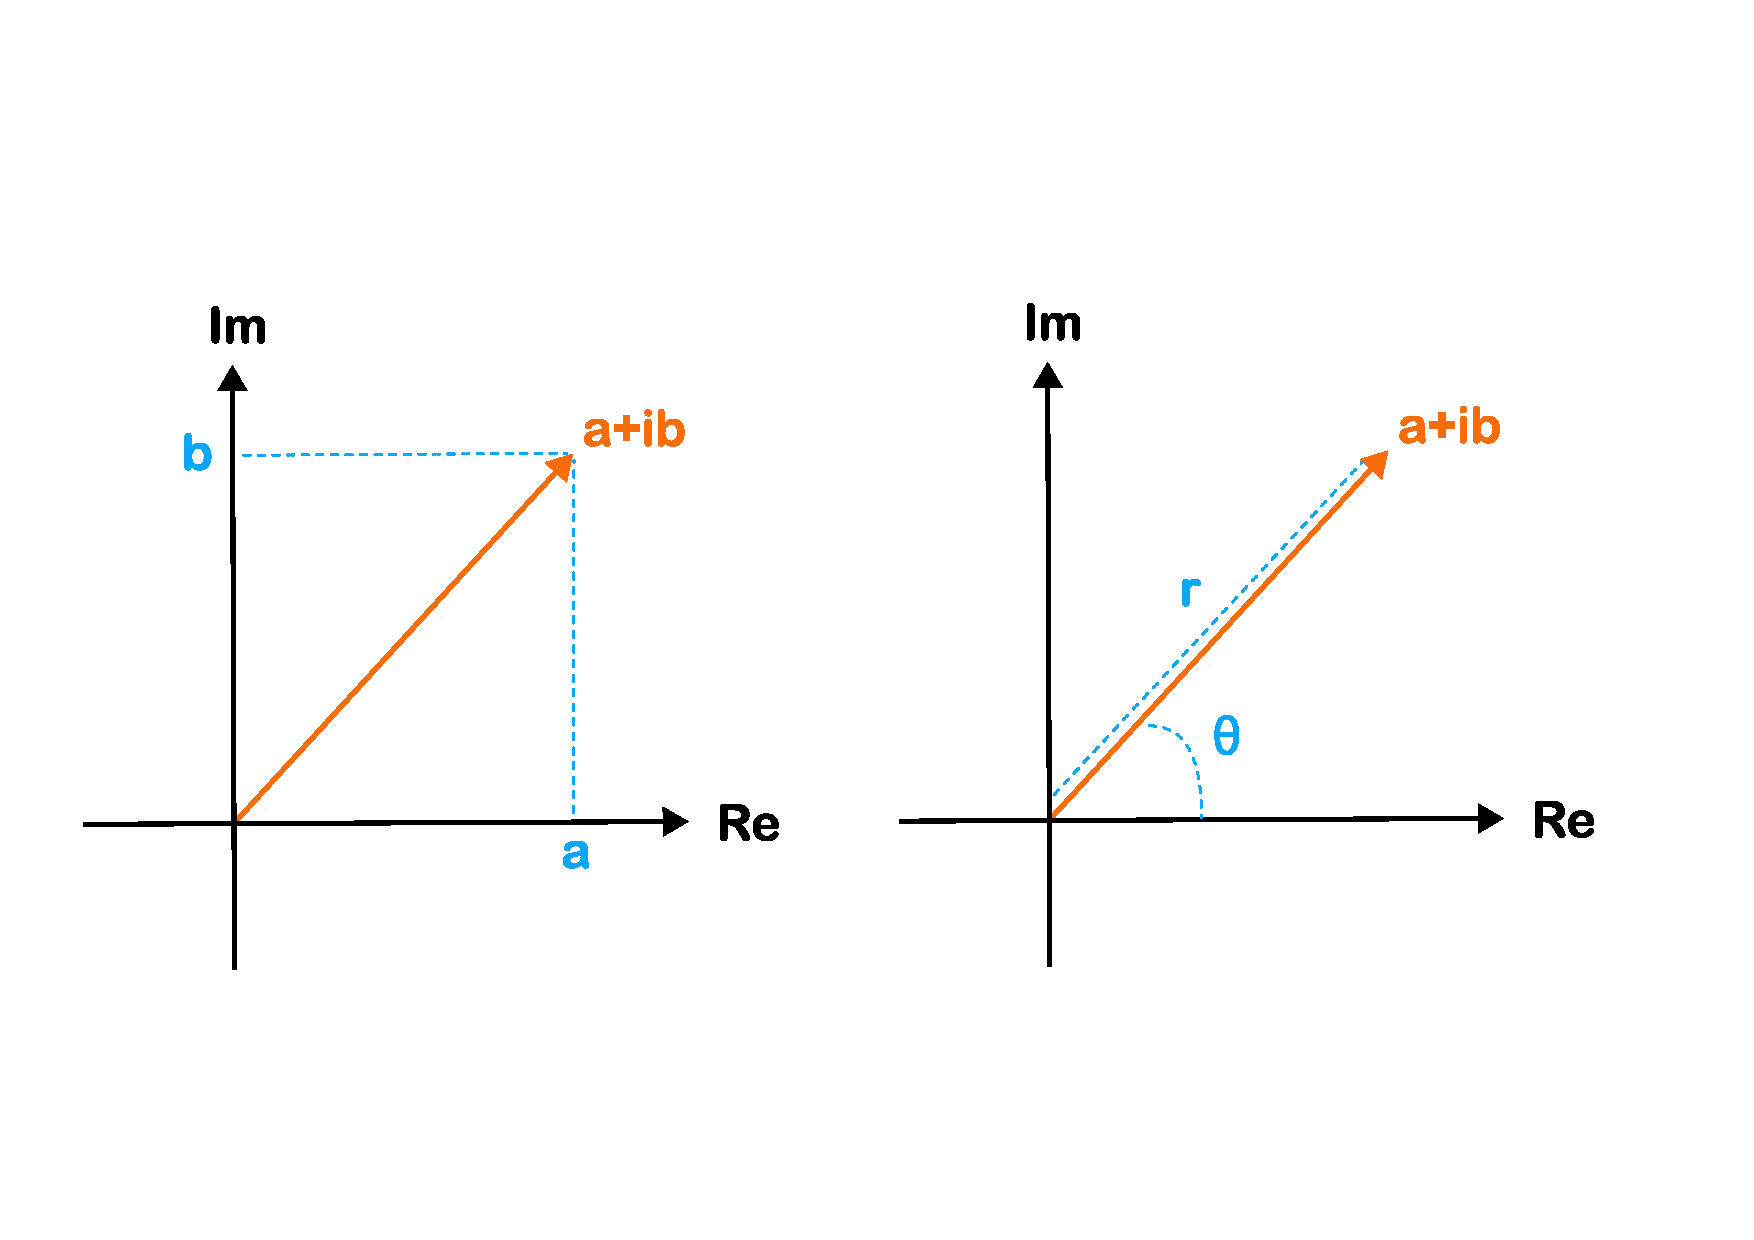
\includegraphics[width=.7\textwidth]{Lecture0Figs/ComplexPlane.pdf}
    \caption{The complex number $z=a+ib$ represented in both Cartesian and polar coordinates as a vector on the complex plane.}
    \label{fig:complex_plane}
\end{figure}

\subsection{Euler's Equation}
This representation becomes particularly powerful when we consider \textbf{Euler's equation}, which states that
\begin{equation}
    e^{i\phi}=\cos\phi+i\sin\phi.\nonumber
\end{equation}
This relationship can be verified by relating the Taylor series expansion of $e^{i\phi}$ with the expansions of $\sin\phi$ and $\cos\phi$. Using this equation and our previously defined relations for $r$ and $\theta$, we can represent any complex number as \begin{equation}
    z=re^{i\theta}\nonumber
\end{equation}
As will be seen in the next section, this representation makes multiplication and division of complex numbers far easier.


\subsection{Matrix Conjugate Transpose}
Now that we are familiar with complex numbers, we can define the matrix \textbf{conjugate transpose}. Given a matrix $A \in \mathbb{C}^n$, this is defined as
\begin{align}
    \textbf{A}^\dagger = \left(\textbf{A}^\textrm{T}\right)^\ast =
    \begin{pmatrix}
        a_{11}^\ast & a_{21}^\ast \\
        a_{12}^\ast & a_{22}^\ast
    \end{pmatrix} \nonumber
\end{align}
If a matrix's conjugate transpose equals its inverse ($\textbf{U}^\dagger=\textbf{U}^{-1}$), the matrix is \textbf{unitary} and
\begin{equation}
    \textbf{U}^{-1}\textbf{U}=\textbf{U}^\dagger\textbf{U}=\textbf{U}\textbf{U}^\dagger=\textbf{I}.
    \nonumber
\end{equation}



%\newpage
%\section{Probability Fundamentals}


%\newpage
%\section{Boolean Logic Fundamentals}


%\newpage
%\section{Fourier Transforms Overview}

\newpage
\section{Additional Readings}
\subsection{Linear Algebra}
\begin{itemize}
    \item One of the best textbooks on introductory linear algebra. Highly recommended to get a good \textit{conceptual} understanding of linear algebra:\\
    {\footnotesize \url{http://math.mit.edu/~gs/linearalgebra/}}
    \item Strang chapter on eigenvalues and eigenvectors:\\ {\footnotesize \url{https://math.mit.edu/~gs/linearalgebra/ila0601.pdf}}
    \item For a basic overview of vectors and matrices as well as some of their properties:\\ {\footnotesize\url{https://web.stanford.edu/class/nbio228-01/handouts/Ch4_Linear_Algebra.pdf}}
    \item A good visual blog post and videos on eigenvalues and eigenvectors:\\ {\footnotesize \url{https://towardsdatascience.com/eigenvectors-and-eigenvalues-all-you-need-to-know-df92780c591f}}
    \item Wikipedia, a good description of eigenvectors and eigenvalues as well as applications to different disciplines: \\ {\footnotesize \url{https://en.wikipedia.org/wiki/Eigenvalues_and_eigenvectors}} 
    
    
\end{itemize}

\subsection{Complex Numbers}
\begin{itemize}
    \item 18.03 course notes on complex numbers:\\ {\footnotesize \url{https://ocw.mit.edu/courses/mathematics/18-03-differential-equations-spring-2010/readings/notes_exe/MIT18_03S10_c.pdf}}
    \item Wikipedia: \\ {\footnotesize \url{https://en.wikipedia.org/wiki/Complex\_number}}
    \item Detailed explanation of complex number manipulation: \\
    {\footnotesize \url{https://www.mathsisfun.com/numbers/complex-numbers.html}}
\end{itemize}

\subsection{Probability}
\begin{itemize}
    \item 6.041 Introduction to Probability Textbook (here is a PDF link to the first chapter, which covers most of the relevant content for this course):\\ {\footnotesize \url{http://www.athenasc.com/Ch1.pdf}}
    \item 6.041 Lecture Notes: \\ 
    {\footnotesize \url{https://vfu.bg/en/e-Learning/Math--Bertsekas_Tsitsiklis_Introduction_to_probability.pdf}}
\end{itemize}


\end{document}